%%%%%%%%%%%%%%%%%%%%%%%%%%%%%%%%%%%%%%%%%
% Thin Sectioned Essay
% LaTeX Template
% Version 1.0 (3/8/13)
%
% This template has been downloaded from:
% http://www.LaTeXTemplates.com
%
% Original Author:
% Nicolas Diaz (nsdiaz@uc.cl) with extensive modifications by:
% Vel (vel@latextemplates.com)
%
% License:
% CC BY-NC-SA 3.0 (http://creativecommons.org/licenses/by-nc-sa/3.0/)
%
%%%%%%%%%%%%%%%%%%%%%%%%%%%%%%%%%%%%%%%%%

%----------------------------------------------------------------------------------------
%	PACKAGES AND OTHER DOCUMENT CONFIGURATIONS
%----------------------------------------------------------------------------------------

\documentclass[a4paper, 11pt]{article} % Font size (can be 10pt, 11pt or 12pt) and paper size (remove a4paper for US letter paper)

\usepackage[protrusion=true,expansion=true]{microtype} % Better typography
\usepackage{graphicx} % Required for including pictures
\usepackage{wrapfig} % Allows in-line images
\usepackage{hyperref}
\usepackage{listings}
\usepackage[utf8]{inputenc}
\usepackage[english]{babel}
\usepackage{cite}
\usepackage{url}
\usepackage{caption}
\usepackage{subcaption}
\usepackage{geometry}
\usepackage{marginnote}
\usepackage{mathpazo} % Use the Palatino font
\usepackage[T1]{fontenc} % Required for accented characters
\linespread{1.05} % Change line spacing here, Palatino benefits from a slight increase by default

\graphicspath{ {images/} }
\lstset{
	numbers=left,
	breaklines=true,
	tabsize=2,
	basicstyle=\footnotesize\ttfamily
}
\makeatletter
\renewcommand\@biblabel[1]{\textbf{#1.}} % Change the square brackets for each bibliography item from '[1]' to '1.'
\renewcommand{\@listI}{\itemsep=0pt} % Reduce the space between items in the itemize and enumerate environments and the bibliography

\renewcommand{\maketitle}{ % Customize the title - do not edit title and author name here, see the TITLE block below
\begin{flushright} % Right align
{\LARGE\@title} % Increase the font size of the title

\vspace{50pt} % Some vertical space between the title and author name

{\large\@author} % Author name
\\\@date % Date

%\vspace{40pt} % Some vertical space between the author block and abstract
\end{flushright}
}

%----------------------------------------------------------------------------------------
%	TITLE
%----------------------------------------------------------------------------------------

\title{\textbf{A Better Browser}\\ % Title
Chasing performance, extensibility, and security} % Subtitle

\author{\textsc{Brooks Mershon} % Author
\\{\textit{Duke University}} % Institution
\\{\textit{CS 342s}}} % Institution

\date{\today} % Date

%----------------------------------------------------------------------------------------

\begin{document}

\maketitle % Print the title section


%----------------------------------------------------------------------------------------
%	ABSTRACT AND KEYWORDS
%----------------------------------------------------------------------------------------

%\renewcommand{\abstractname}{Summary} % Uncomment to change the name of the abstract to something else


%\hspace*{3,6mm}\textit{Keywords:} lorem , ipsum , dolor , sit amet , lectus % Keywords

\begin{abstract}
	This paper briefly covers the history of each major web browser and discusses several vulnerabilities against which modern browsers must be designed to protect users. The architecture of the Chrome extension system is presented as an elegant solution for meeting a modern web browser's need to be secure while running third-party extensions on arbitrary web pages. The author's own Chrome extension, which was developed for a database systems course, is used to illustrate the way Chrome's extension system allows for third-party contributions to improve users' browsing experience without compromising Chrome's security. Considerations for the future of browser development are given in light of Chrome's preeminence as a modern web browser.
\end{abstract}

\eject

\tableofcontents
%----------------------------------------------------------------------------------------
%	ESSAY BODY
%----------------------------------------------------------------------------------------

\eject

\section{What is a Web Browser? }

A web browser is just a software application, but it is a very special piece of software. First and foremost, a web browser is built for humans to use and interact with---often for many hours per day! Its purpose is to retrieve and present the wealth of information to be found on the World Wide Web. You can think of the web browser as a portal to the internet, for its job is to take you where you want to go and show you what you want to see. Creating a software application that can do this well is no small feat. For this reason, among many others, there have emerged only a handful of browsers over the past several decades that are in regular use. Among the major browsers in use today are Chrome, Firefox, Safari, Opera, and Internet Explorer.

There are two significant functionalities that any web browser must provide: the ability to retrieve a resource and the ability to render its content. Both of these functionalities are closely tied to standards which have developed over time. After all, the web depends on standardized methods of communicating and representing information. These standards certainly evolve and change over time as new ideas emerge, pushing web browsers to evolve along with them. Let us consider the basics of the web browser's functionality:

\begin{itemize}
	\item \textbf{Retrieval.} Suppose you give the browser the \textbf{URL} \url{https://www.reddit.com/}. The \textbf{URI} (Uniform Resource Identifier) is the \textit{https:} prefix of the Uniform Resource Locator. This prefix defines a protocol to use in order to find the resource found at \url{reddit.com}. The internet protocol suite is a standard around which all web browsers must develop.
	
	\item \textbf{Rendering}. Once the information found at \url{https://www.reddit.com/} has been retrieved, it must be displayed or \textbf{rendered} by the browser. Here, too, we find standards to which a successful browser must form. \textbf{HTML} (Hypertext Markup Language) is just one example of a standard specifying the way information on the internet can be organized and rendered. There happen to be a few \textit{acid tests} that have been developed so that the way browsers render content can be tested uniformly). These tests consist of a series of complex operations which make use of the specifications set forth by the World Wide Web Consortium, the Unicode Consortium, ECMA, to name a few. \textbf{Acid2}, for example, constructs a smiley face when a browser successfully navigates a series of tests for HTML and CSS implementations. \cite{AcidT95:online}
	
	\textbf{Acid3} is the most recent test developed by The Web Standards Project, a grassroots coalition founded in 1998. \cite{TheWe20:online} Figure \ref{fig:acid2-chrome49} shows a successful render of the Acid2 test by the author's current version of the Chrome browser (version 49). A failure is easy to recognize in Figure \ref{fig:acid2-opera8-fail}, which shows Opera 8 unsuccessfully rendering the Acid2 test. A more modern Acid3 test verifies compliance with a much wider range of technologies, including but not limited to:
	
	\begin{enumerate}
		\item DOM (Document Object Model, or the scenegraph of a web page)
		\item Unicode UTF-8 (character encoding)
		\item HTML 4.0 (structure of a web page)
		\item CSS (Cascading Style Sheets, or the appearance of the HTML's structure)
		\item SVG (Scalable Vector Graphics)
		\item EcmaScript (JavaScript)
		\item HTTP (Hypertext Transfer Protocol)
	\end{enumerate}
	
\end{itemize}

\begin{figure}
	\centering
	\begin{subfigure}[b]{0.3\textwidth}
		
\includegraphics[width=\textwidth]{acid2}
		\caption{Chrome 49 (February 2016) rendering Acid2.}
		\label{fig:acid2-chrome49}
	\end{subfigure}
	~ %add desired spacing between images, e. g. ~, \quad, \qquad, \hfill etc. 
	%(or a blank line to force the subfigure onto a new line)
	\begin{subfigure}[b]{0.3\textwidth}
		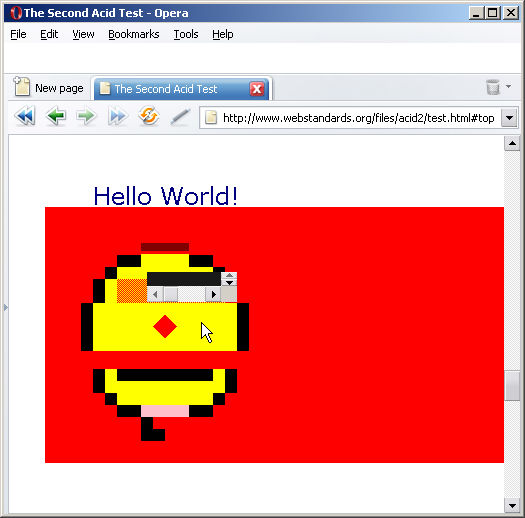
\includegraphics[width=\textwidth]{acid2-opera-fail}
		\caption{Opera 8 (April 2005) fails Acid2 when first released.}
		\label{fig:acid2-opera8-fail}
	\end{subfigure}
	~
	\begin{subfigure}[b]{0.3\textwidth}
		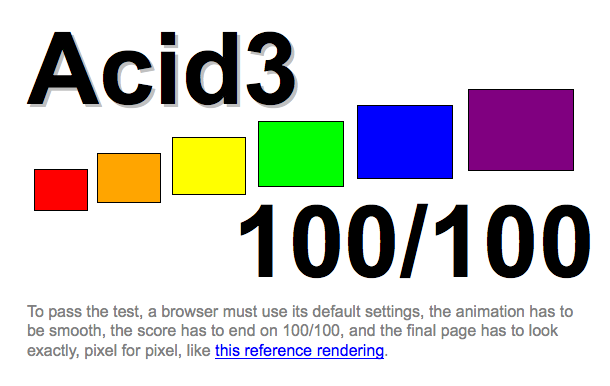
\includegraphics[width=\textwidth]{acid3-firefox44}
		\caption{Firefox 44 (January 2016) rendering Acid3.}
		\label{fig:acid3-firefox}
	\end{subfigure}
	\caption{Acid2 and Acid3, launched in April 2005 and March 2008, respectively.}\
\end{figure}

These \textit{acid tests} should in theory verify the correct interaction of many complex technologies implemented by the browser, particularly those implemented in a browser's \textbf{layout engine}. The most recent test, Acid3 (see Figure \ref{fig:acid3-firefox}), can quantify the extent to which a browser succeeds in passing the rendering test. All major browsers now achieve a perfect 100/100 score on Acid3, despite developers' criticisms of the cherry-picked selection of features this test touches on. Acid2 demonstrates the catastrophic failure of some tests through its visual output (does the output look like \ref{fig:acid2-chrome49} or not?). That web browsers are constrained by their need to conform to a wide array of standards can be appreciated by these visual tests, though there are less visual aspects which are tested by other frameworks as well. Part of the beauty of the web browsers that have emerged is the proliferation of different technical strategies for providing the base functionality of retrieval and rendering.

But browsers have grown beyond merely retrieving and rendering (as fast and reliably as possible). Modern browsers add to this functionality by providing the means to \textit{extend} their features by incorporating other software applications, often written by third parties (i.e., \textit{not} Google, Mozilla, Apple, or Microsoft). In this way, the modern browser has evolved beyond a monolithic \textit{software application} to represent a platform for continual innovation, its features expanding to fit the needs and desires of users. If browsers already faced a daunting task in providng a secure experience in the early days, the modern browser's ability to be extended by third-parties presents a new frontier of vulnerabilities and security concerns which must be addressed.

\section{A Brief History of Browsers}

The history of browser development can be understood in terms of the parallel timelines of innnovations made by various companies and their products. There are early entrants and late entrants in the great browser race, each adopting good ideas from others as the internet continued to evolve. \cite{evolution-of-the-web}

\subsection{Mosaic (1993)}

Sir Tim Berners-Lee, known as the inventor of the World Wide Web, kicked off this browser race with a piece of software that could view documents on the Web. The browser didn't have many of the amenities we appreciate today, such as bookmarks and other forms of persistent browsing data, but it was graphical and user friendly, and that counts for a lot. \cite{Frequ89:online, evolution-of-the-web}

\subsection{Netscape (1994)}

Netscape Communications Corporation, inspired by Mosaic, created the Netscape web browser in 1994. As far as rendering goes, Netscape introduced on-the-fly rendering, where a page is rendered as it downloaded, rather than all at once. Slow as download speed were at the time, the incremental rendering of Netscape made browsing a more tolerable experience for 1990s users. \cite{Remem57:online}

The Netscape browser was first to support JavaScript, a cobbled together, untyped, interpreted language that, despite being devoped in \textit{10 days} by Netscape employee Brendan Eich (as rumor has it), has managed to become the lingua franca of computation on the web. JavaScript brings web pages to life, allowing for dynamic content, such as mouse-click driven interaction (e.g. play sound, fade colors, move text). Today, JavaScript is used by every browser to perform some heavy duty lifting: many JavaScript libraries exist for performing scientific computing, rendering 3D models, and transforming large amounds of data in the browser. Netscape actually created a language that became a \textit{standard}: ECMAScript codifies the exactly specifications for the language so that it may be implemented correctly everywhere; indeed, this standard does change gradually over time, with new language features being introduced this very year as browsers adopt ES2015. For better or worse, JavaScript is used to do good and evil on the web, its roots tracing back to the Netscape days of dynamic web pages. \cite{evolution-of-the-web}

\subsection{Opera (1996)}

In addition to being a popular browser for mobile devices, Opera introduced a few features that other browsers have subsequently adopted, some of which are related to user privacy:

\begin{enumerate}
	\item \textbf{Multiple tabs.} A way for organizing browsing experiences. Of course, multiple tabs are not enough: Chrome will introduce tabs as a model for browsing in which each tab is its own separate, sandboxed process. In this way, Opera introduced the experience of tabbing, and Chrome will later revolutionize the implementation of tabbed browsing experiences.
	\item \textbf{Pop-up blocker.} Not only are pop-ups annoying, they can potentially lead to phishing attacks which lure users to click links which take them to sites that are not what the user expected them to be. \cite{5feat81:online} Perhaps Brendan Eich, former CEO of Mozilla, will fix that with the Brave browser. \cite{Brave19:online}
	\item \textbf{Delete private data}. An HTTP cookie is a small piece of plain text---no executable code. However, these cookies are used all over the place by sites wishing to maintain stateful data about a user. \cite{Whata43:online} Sometimes, these cookies contain sensitive information, or at the very least leave breadcrumbs indicating what a user has done while using the browser. Opera thought it would be nice to be able to get rid of these, for privacy's sake.
\end{enumerate}

According to Opera, there are over 350 million devices using the browser. \cite{About26:online} A significant portion of these devices are mobile computing platforms. In 2006, the Nintendo DS used a version of Opera and its mobile layout engine. \cite{Givin8:online} Opera's use as a mobile browser suggests the potential for niche browsers to evolve for particular products despite enjoying a comparatively small proportion of all browser usage.

\subsection{Internet Explorer (1995)}

Internet Explorer has needed to maintain an ability to enter "quirks mode" so that websites designed to render appropriately for older versions that were not standard-compliant will render appropriately when Internet Explorer \textit{is} standards-compliant. This alone should suggest the rather rocky road that Internet Explorer has traveled as it matured. Internet Explorer has been the bane of many web developers' existence because it is idiosyncratic in its approach to technologies like CSS, HTML, and even the JavaScript language, among others critical web standards.

From a security standpoint, Internet explorer has been the target of many vulnerabilities which take advantage of certain plug-ins that it uses, more or less on account of the fact so many people were using the browser from 1997 onward. 1998 happened to be the year Microsoft became involved in an antri-trust trial, largely as a result of its choice to bundle internet explorer with Windows. \cite{Inter45:online}

\subsection{Firefox (2004)}

Like Chrome, Firefox is known for being standards-compliant throughout most of its history. Also like Chrome, Firefox uses a sandbox security model. Firefox is perhaps most notable as a browser for the culture Mozilla carries with it. In 2013, Mozilla was recognized as the most trusted internet company for privacy. \cite{Mozil33:online}

\subsection{Safari (2005)}

Apple has been criticized in the same vein as Microsoft because of its promotion of its own browser. \cite{Mozil34:online}. Safari is about as proprietary as a browser can get, and with this comes the risk of browser exploits which could have been detetected and patched if more eyes were on the code. \cite{brows80:online} The culture of Apple naturally puts Safari in a different position than Firefox and Chrome, because both Mozilla and Google have made all or almost all of the source for their respective browsers open source. \cite{Googl14:online}

\subsection{Chrome (2008)}

In 2008, the Chrome Team at Google decided to start from scratch. \cite{chrome-comic} There are a few notable features which make Chrome stand out as a modern browser:

\begin{itemize}
	\item \textbf{Web standards support.} Unlike Internet Explorer, Chrome has always passed Acid1, Acid2, and Acid3 with the highest scores. There is a JavaScript conformance test called ECMAScript Conformance Test 262, for which Chrome fails only 10 out of 11,578 tests, while Firefox fails nearly 200 and Internet Explorer 9 failed over 600. \cite{Googl45:online}
	\item \textbf{Sandboxing.} Chrome makes a new process for each tab that a user creates. Each process has no means for interacting with the user's machine outside of the Chrome browser. \cite{Googl36:online}
	\item \textbf{Auto-updates}. Stale browsers are a vulnerability, because the web evolves and people discover ways to exploit browsers. Chrome updates not only Chrome's own code, but also a list of blacklisted websites which can help warn users that phishing attacks or other malicious activity has been found from a particular site.
	\item \textbf{Extended Validation Certificate.} Chrome can show a little green lock in the browser to indicate that a public key certificate has been verified for the site you are visiting. This is a handy way to know \texttt{https://www.wellsfargo.com/} is really Wells Fargo.
\end{itemize}

\eject

\section{Browser Vulnerabilities}

\subsection{Injection}

If a script on a web page evaluates data which is untrusted and may in fact be a command (e.g., JavaScript \texttt{eval()}), the browser or even other processes in the user's machine can be made to execute unintended commands. This vulnerability is closely related to Randal Munroe's famous \textit{Exploits of a Mom} XKCD comic. \cite{xkcd:10:online}

\subsection{Cross-Site Scripting (XSS)}

A web page can force a browser to execute malicious JavaScript code. Since there is no way to know whether a script is malicious or not, there is a real risk in a browser being redirected to malicious sites. Moreover, XSS attacks rely on making a browser execute arbitary code capable of capturing or modifying forms or sensitive information on the web page. \cite{Top1046:online}

\subsection{Direct Object References}

Internal implementaition objects, possibly with access to powerful browser capabilities such as file system access, are inadvertently exposed to web pages through exact references to objects. One way to think of this attack is as follows: you have given a pile of keys for unlocking powerful APIs in the browser to a web page. \cite{Top1046:online}

\subsection{Plug-ins}

Plug-ins expose APIs to web pages which may or may not choose to use them. Examples of plug-ins include the ability to render PDF and Flash media types. \cite{38394}

\subsection{Extensions}

Plug-ins expose additional APIs to the browser and help provide the tools a web page may require to render media types like PDF and Flash. Extensions, however, interact with the content of web pages without the web page requesting them to do so. Because extensions are closely tired to the browser's API, they are a natural vector for attacks which aim to exploit non-malicious third-party extensions. Of course, if an extension is itself malicious, it is incumbent on the user to avoid installing it or the extension marketplace's curation team to ensure it is not available.

\subsection{Languages}

JavaScript is not JavaScript across all browsers. According to Mozilla's Developer pages:

\begin{quotation}
JavaScript (JS) is a lightweight, interpreted, programming language with first-class functions. Most well-known as the scripting language for Web pages, many non-browser environments also use it, such as node.js and Apache CouchDB. JS is a prototype-based, multi-paradigm, dynamic scripting language, supporting object-oriented, imperative, and functional programming styles. Read more about JavaScript. \cite{JavaS76:online}
\end{quotation}

The specification for the JavaScript language comes from Ecma international (and has nothing to do with the Java programming language). The JavaScript specification is supported across all browsers but not necessarily implemented using the same underlying engines. Naturally, the potential for security exploits arises from these implementations.


\section{Chrome Extensions}

Chrome extensions build on top of Chrome's innovative process-per-tab, sandboxed computing model by creating an architecture which enforces secure development practices for third-party extensions. The future of rich browsing experiences depends on the ability to extend a browser in unimaginably creative ways. The security of Chrome, which stands out among the major browsers as one of the more advanced, depends on maintaining a high level of security and \textit{robustness} while introducing \textit{more software} that may be potentially buggy and subject to unintended vulnerabilities. From the  Chrome developer page:

\begin{quotation}
	Extensions are small software programs that can modify and enhance the functionality of the Chrome browser. You write them using web technologies such as HTML, JavaScript, and CSS. \cite{Whata95:online}
\end{quotation}

One year after Google released Chrome in December 2008, a new kind of extension architecture was introduced to the browser. The Chrome extension system was designed to address many of the security concerns seen in Firefox extensions. Chief among the problems facing the Firefox extension system was the total privilege most extensions enjoyed. Every Firefox extension, whether it needed to or not, was able to run arbitrary code on a user's machine because it had access to all of the powerful browser functionality by default. \cite{38394} A browser usually has the ability to run arbitrary code on a user's machine, but modern browsers are written by security experts who can continually update the browser in light of any vulnerabilities that surface. \cite{34924} Firefox extensions ran with the full privileges of a browser before Chrome extensions were introduced. In most cases, they were written by third-parties who are \textit{not} security experts. Chrome extensions limit the security vulnerabilities inherent to third-party extensions by not only granting the highest privileges to extensions that truly require it, but also isolating extension internals and special browser components from interactions with arbitrary web pages.

\subsection{Privilege Gap}
The Chrome extension architecture recognizes the gap between what a browser is capable of and the capabilities most extensions actually require. Chrome can access a user's file system, for example, as well exchange messages with native applications on a user's machine---that's about as privileged as you can get. \cite{38394}

Many extensions are modest in the privileges they require. One particular Chrome extension, named \textit{Cloud to Butt Plus}, replaces occurences of the phrase \textit{the cloud} in a web page with \textit{my butt}. \cite{Cloud45:online} Useful or not, this extension would enjoy the full privileges of the Firefox browser years ago and represent a serious security risk. One can imagine that part of the extension's functionality entails querying the DOM (Document Object Model) using the element selector API. If a malicious website were to replace these DOM selectors with forged objects that look like the objects the extension expects them to be, but in fact have different (nefarious) side effects, a browser could be tricked into providing a means of obtaining references to internal objects. That's bad, because the extension could make the browser modify a user's machine in unexpected ways---this is the very worst case scenario of a browser exploitation.

In this way, \textit{cloud-to-butt} is at risk of subjecting an extension user to a cross-site scripting attack. Instead, under the Chrome system, this particular extension is effectively sandboxed and its privileges taken away so that there is no way for a malicious website to compromise the Chrome browser with this extension. This extension only requires the ability to modify the DOM of an arbitrary web page. Although interacting with arbitray web pages exposes an application to a large suite of vulnerabilities, this particular extension is simply not granted the privileges required to do anything more than (hilariously) modify a web page. Chrome protects the browser from security vulnerabilities by creating a platform that encourages developers to build secure extensions by default. We can better understand the design philosophy of Chrome's extension system by examining the structure of a Chrome extension written by the author.

\subsection{Case Study | WikiBlocks Chrome Extension}

There are three concepts that best describe the Chrome extension design philosophy: \textit{least privilege}, \textit{privilege separation}, and \textit{strong isolation}. \cite{38394} A Chrome extension is, after all, just a third-party software application which happens to augment the Chrome browser. In order to illustrate the way in which the Chrome extension system mitigates security risks introduced by third-party extensions, we will consider the capabilities of the author's own fully-functioning prototype Chrome extension developed for a database systems course taught at Duke University.

The WikiBlocks project is a Chrome extension and backend system that finds relevant visualizations for a STEM-related Wikipedia article. The visualizations are GitHub gists rendered by Mike Bostock's \texttt{bl.ocks.org} viewer, for which a burgeoning ecoystem of STEM-related visualizations has emerged (most of which are written in JavaScript and use Bostock's visualization library, called D3). The backend system consists of a database and server responsible for searching an ever-growing index of visualizations and maintaining associations between conceptually related visualizations as they are created and updated. Figure \ref{fig:wikiblocks} shows a Wikipedia page for \textit{Adjacency matrix} and three results presented by the extension pop-up which direct the user to running examples on \texttt{bl.ocks.org}. Because the WikiBlocks project is first and foremost designed to augment a user's Wikipedia experience, the introduction of an extension to the user's browser which activates on just Wikipedia pages should be a boon to individuals looking to visualize abstract concepts related to science, technology, engineering, or math. However, interaction with arbitrary webpages, even those coming from Wikipedia, presents an opportunity for WikiBlocks to create a security vulnerability for Chrome users who install it.


\begin{figure}[h]
	\centering
	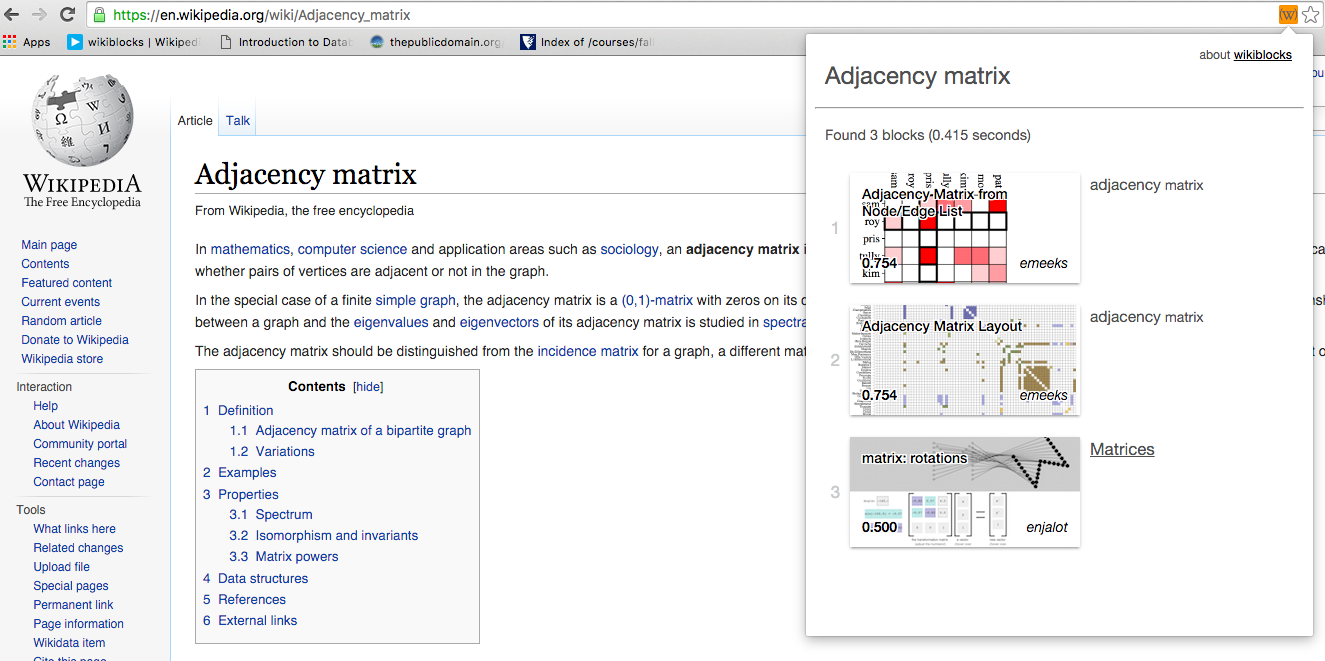
\includegraphics[width=\textwidth]{wikiblocks-adjacency}
	\caption{Author's \textit{WikiBlocks} Chrome extension developed for a database systems course taught at Duke University.}
	\label{fig:wikiblocks}
\end{figure}


\eject

Figure \ref{fig:rips-complex} shows an interactive visualization running on \texttt{bl.ocks.org} that illustrates a STEM-related concept that a user may wish to visually engage while visiting a Wikipedia article for \textit{Vietoris-Rips complex}. The WikiBlocks extension discovers and adds such visualizations to a database when a user with the extension installed visits them on \texttt{bl.ocks.org}. When the extension is triggered on a Wikipedia article, it attempts to find relevant results by querying the database using information gleaned from the article's web page.

\begin{figure}[h]
	\centering
	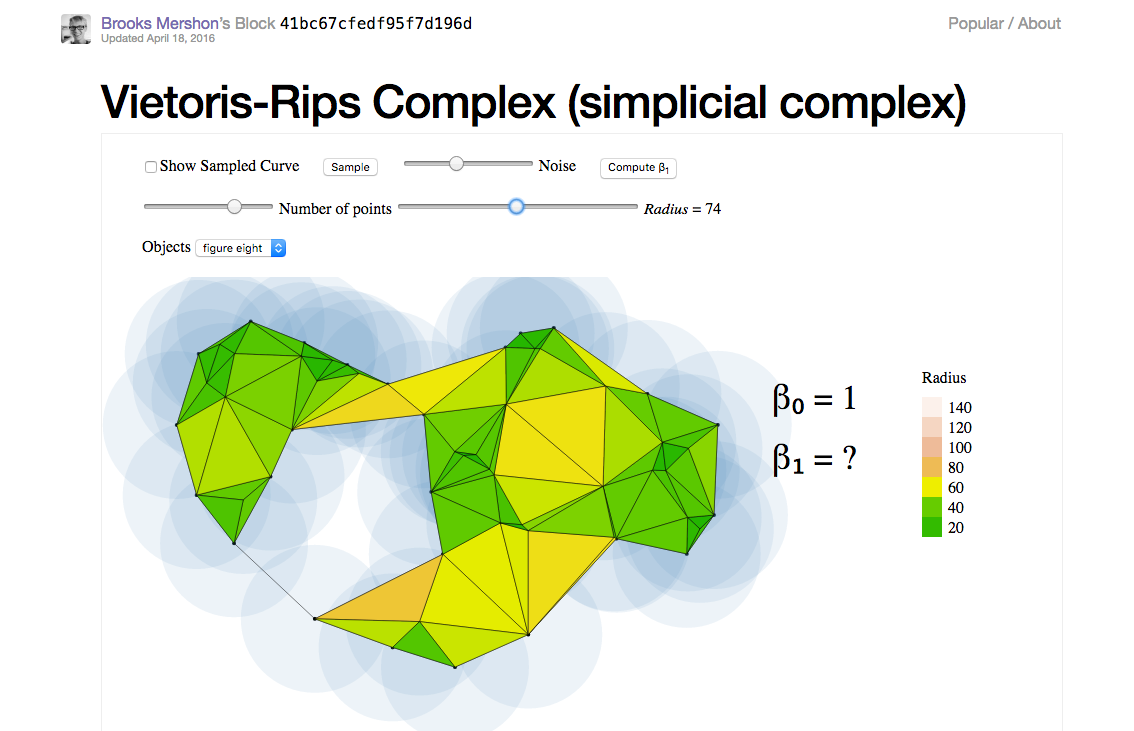
\includegraphics[width=\textwidth]{rips-complex}
	\caption{The author's visualization of the Vietoris-Rips complex running on \texttt{bl.ocks.org}. The WikiBlocks extension provides a thumbnail and link to this visualization when a user clicks the WikiBlocks icon in the toolbar while visiting a Wikipedia article related to simplicial complexes or topology.}
	\label{fig:rips-complex}
\end{figure}

\subsection{Least Privilege}.

The Wikiblocks extension, like all Chrome extensions, explicitly delares the privileges it requires in a file called \texttt{manifest.json}. \cite{wikib0:online} The following snippet of this file declares the extension's intention to use the Chrome API for accessing a user's active tab, as well as the ability to make cross origin requests \textit{only} to the origin at which the WikiBlocks server is located. 

\begin{lstlisting}
"permissions": [
	"activeTab",
	"http://wikiblocksalpha.elasticbeanstalk.com/*"
],
\end{lstlisting}

Many more permissions could be requested and a user installing this extension would be warned that they will be available to the extension. Since WikiBlocks only needs to know which tabs are active (search results can be maintained across several open tabs!), as well as the ability send requests to a single origin other than the user's own machine, these are the only declared permissions. It is easy to see where the \textit{manifest.json} name comes from. It's a JavaScript Object Notation blob that tells Chrome which privileges your extension requires. There's no way to fake the manifest. The manifest is the law.

The vulnerability of this extension to cross-site scripting attacks which might cause the browser to send HTTP requests to any origin other than the one listed in the manifest file has been eliminated. Moreover, the only powerful API that the extension will be permitted by Chrome to use is the \textit{activeTab} API. WikiBlocks is allowed to do only what it needs to; a malicious web page cannot force WikiBlocks to do much harm to the user. Could an injection attack be launched against the WikiBlocks database? Possibly, but the user of the WikiBlocks Chrome extension certainly does not risk a web page causing the extension to affect his or her own browser settings, persistent browser storage, or other processes on the host machine.

\subsection{Privilege Separation}. The WikiBlocks extension has three main components: a content script, an extension core, and an HTML page which serves as the popup a user sees when they click the WikiBlocks icon in their toolbar. These components have different privileges and their separation ensures that the arbitrary web pages that WikiBlocks may interact with will have a difficult time fooling the extension into doing something bad for a Chrome user. But just how are they separated? For one thing, they each run in separate processes. This means that JavaScript object references cannot be exploited to in a way that would allow a malicious web page to gain access to the powerful Chrome browser API. The name of the game for coordination between the extension components is \textit{messaging}.

\begin{itemize}
\item \textbf{Content script(s).} This script runs in a separate process from the one running any scripts found on a web page. It's called a "content" script because it is inserted into a web page. WikiBlocks uses a content script to find article information needed to query the database for a relevant gist (Figure \ref{fig:wikiblocks-quicksort}). The concent script has only one way to interact with the rest of the extension: send a message. Consider the following snippet from the WikiBlocks concent script:
	
\eject
	
\begin{lstlisting}
chrome.runtime.sendMessage({method: "performSearch", page: page}, function(results) {
	//data may have an error, which must be evaluated
	data = results;
	sendResponse(results);
	chrome.runtime.sendMessage({method: 'ready'});
});
\end{lstlisting}	

What is happening here? The script is shouting (asynchronously) to the rest of the extension that whoever is responsible for performing a search for the current Wikipedia article should go perform that search with the information found by the content script. When a response is received from whomever performs the search, the content script shouts another message to whomever is listening, saying that results are ready. The reason for this message passing becomes clear when we consider the inability of a content script to execute cross-origin requests, by Google's design. A Wikipedia page cannot force the content script to make a request to another origin, nor can it force the content script to use any other \texttt{chrome.runtime.*} API besides sending a message and checking what the URL of the page is. The content script can only query and modify the Wikipedia page and then send any messages it wants to the other extension components that may be listening.

\item \textbf{Extension core (event listeners)}. The extension core can either be a long-running script which maintains state across the life of the extension, or an event page that is loaded only when needed. WikiBlocks uses the latter model, with a script whose sole job is to define event listeners for any message sent by either the content script or the popup page. The extension core, or in the WikiBlocks extension, \texttt{eventPage.js}, is able to use all of the \texttt{chrome.runtime.*} API and serves the purpose of coordinating the content script and popup. Consider the single event listener which allows the event page to respond with an appropriate handler to any message from either the content script or the popup script which accompanies the popup page that the user can launch:

\eject

\begin{lstlisting}
// ... functions not shown

var handlers = {
	'havePage': havePage,
	'ready': ready,
	'getPage': getPage,
	'getResults': getResults,
	'performSearch': performSearch,
	'foundGist': foundGist,
	'clickedGist': clickedGist
}

// ... functions not shown

chrome.runtime.onMessage.addListener(function(message, sender, sendResponse){
	if(handlers.hasOwnProperty(message.method))
		return handlers[message.method].call(null, message, sender, sendResponse);
	else
		return false; // Not expecting a response
});
\end{lstlisting}

The extension core is the most privileged component of the WikiBlocks extension: it is able to send a cross-origin XMLHttpRequest to the WikiBlocks server, which is a white-listed origin with which the extension has explicitly declared a need to communicate.

\item \textbf{Popup (HTML and script).} The visual representation of the WikiBlocks Chrome extension is entirely defined by the popup's behavior. Figure \ref{fig:wikiblocks-lab} shows an example of the WikiBlocks popup rendering page results. Searches are performed for a Wikipedia article the moment the content script ships off its parsed information to the extension core and the extension core sends a request to the server. When results have been found, the WikiBlocks icon in the toolbar changes color and a user may choose to click on it to see the search results. What happens if a user clicks on the icon before the results have been found? The user is greeted with a nice loading icon and other useful information. The asynchronous messaging coordinated by the extension core negotiates the messaging between both the content script and the popup to ensure that the popup is updated when search results are available, whether the popup is open or not. The popup, like the content script, runs in its own process and is only able to communicate with the rest of the extension through messages. No strong references to JavaScript objects exist between the three components, and the popup cannot use any other powerful extension API. The Chrome extension system thus ensures that the neither the popup nor the content script offer a vector into exploiting the Chrome browser as a result of bugs in an extension. The extension core is limited by the permissions it requests. An arbitrary web page could only influence the extension through the plain-data sent via \texttt{chrome.runtime.sendMessage()}, which is a rather difficult way to force the extension to compromise the Chrome browser.
\end{itemize}

\subsection{Strong Isolation}. 

The least privilege principle lends the chrome architecture a division of responsability that falls along the three components outlined above: content script, extension core, popup. While the WikiBlocks extension did not make use of native binaries, other extensions may ver well do so. There are several ways in which the Chrome extension system maintains an isolation between web concent and powerful browser capabilities.

\begin{itemize}
	\item \textbf{Origin of resources}. Scripts which do not come from the extension are not run. Extension scripts are packaged into a file when they are distributed to users who install them: all of the resources such as HTML pages and JavaScript files must be loaded from a user's local file system. This prevents a malicious page from swapping in another resource and tricking the extension into running untrusted code. If it's not in the manifest, it is not run. \cite{38394}.
	
	\item \textbf{Isolated Processes.} A separate process is used for the scripts run as content scripts, event handlers (extension core), popup scripts, and possibly native binaries used by the extension. As illustrated by the WikiBlocks example, each of the extension compoents can only interact with one another through messaging: no Object references can be shared because each process runs with its own heap. An attacker cannot chase pointers with the hopes of uncovering references to Chrome browser components or internal extension components which make use of Chrome extension runtime APIs, such as powerful file system access. In fact, Chrome even runs plug-ins in a separate process so that errant plug-ins can be identified and squashed. \cite{20-things} 
\end{itemize}

\begin{figure}
	\centering
	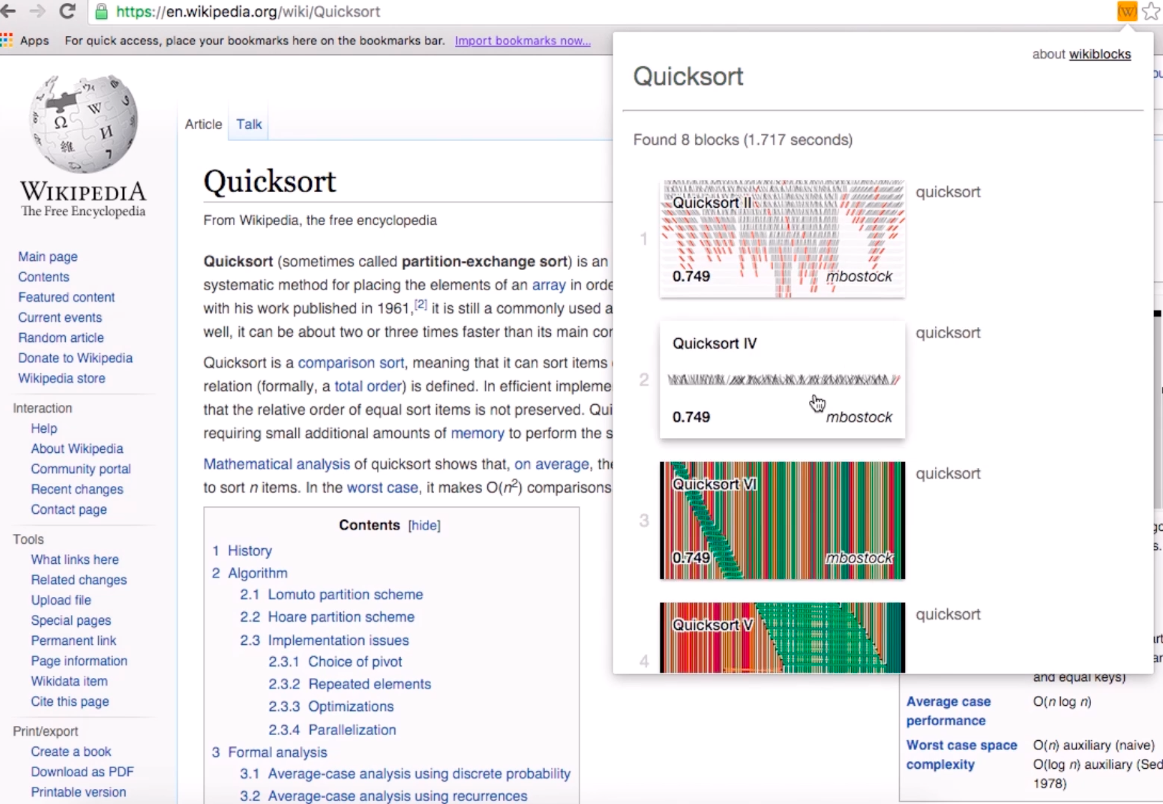
\includegraphics[width=\textwidth]{wikiblocks-quicksort}
	\caption{The content script responsible for parsing the page runs in a separate process from the other scripts which might be present in the Wikipedia page, but has access to the same DOM as any other script running on the web page. This design ensures that a malicious web page cannot use any JavaScript objects in the content script to gain access to the Chrome extension API: no ability to abuse files storage, make cross-origin requests, access tabs, or gain access to sensitive data held in the extension. The content script lives in its own world and can only interact with the Chrome browser by messaging an extension core with more privileges.}
	\label{fig:wikiblocks-quicksort}
\end{figure}

\begin{figure}
	\centering
	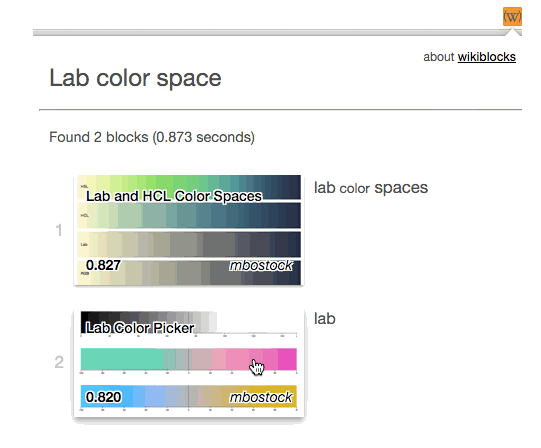
\includegraphics[width=\textwidth]{wikiblocks-lab}
	\caption{The WikiBlocks extension popup is rendered from a small HTML script and controlled by another pre-packaged JavaScript file. The popup can \textit{message} the extension core and present information by updating its own DOM, but otherwise has little power to do any harm. The popup cannot, for example, evaluate in-line scripts (which a malicious attacker might inject), nor can it perform cross-origin requests. It's use of the Chrome runtime API is limited to messaging other more privileged components of the extension.}
	\label{fig:wikiblocks-lab}
\end{figure}

\eject

\section{Looking Forward}

Of the major browsers in use today, Chrome stands out as a modern browser that meets the ever increasing desire for performance and security for desktop browsing experiences. The content of the web becomes richer as browsers are able to compute faster, support libraries developers wish to use, and maintain their security in the face of growing complexity. Chrome's process-per-tab design creates a pleasant browsing experience in which a failures in any single process from either a web page or an errant plug-in cannot bring down all of a user's processes. Other browsers must necessarily provide at least this level of robustness as new iterations are created.

But a browser must also be extensible, and Chrome's extension system demonstrates a solution for incorporating third-party extensions that encourages secure development practices without relying on a developer's ability to foresee complex interactions which result in browser vulnerabilities.

Yet Chrome is not perfect, as much as the author is fond of its screaming V8 JavaScript engine, capable of rendering the computationally intensive visualizations utilized by the WikiBlocks extension. Chrome draws significantly more power from many mobile devices and laptops than does Safari, for example, much to the dismay of users finding themselves without an electrical outlet. Firefox stands to revolutionize the way web pages are rendered with its new layout engine. Servo, unlike current rendering engines, will make use of the GPU to render web pages in parallel, using a new programming language called Rust. \cite{Servo40:online} What Chrome and Firefox's new design demonstrate is the possibility for browsers to evolve by leaps and bounds, not just by incremental improvements.

The famous Chrome Comic illustrated by Scott McCloud paints the journey of Chrome's creation as a clean slate, back to the drawing board development process undertaken at a time when the web was just too good for older browsers. \cite{chrome-comic} Chrome may be a dominant browser now, but who knows what the future of browsers will look like. What should be expected, it seems, are significant changes in form, function, and implementation just like we saw with Chrome's introduction in 2008. Incremental browser improvements give way to new ways to achieve performance while maintaining the security of a browser that users depend on. Chrome seems to have figured out secure extensibility. Perhaps other browsers will teach Chrome a lesson about secure interaction with web technologies in the years to come.

A lot of browser development is concerned with supporting good standards and letting legacy code die out, particularly when legacy code is either slow or vulnerable to exploits. As fast as the web evolves, web standards seem to move at a slower pace, upholding safety at the price of constraining browser development. It is likely that a company like Mozilla will soon produce a new technology which quickly ushers in more secure web standards around which the other browsers will rally.

\eject

\appendix

\section{Appendix}

\subsection{WikiBlocks | manifest file}

\begin{lstlisting}
{
	"manifest_version": 2,
	"name": "WikiBlocks",
	"description": "This extension helps you find ....",
	"version": "1.0",
	"content_scripts": [
		{
			"matches": ["https://en.wikipedia.org/wiki/*"],
			"exclude_matches": [
				"https://en.wikipedia.org/wiki/Main_Page",
				"https://en.wikipedia.org/wiki/*:*"
			],
			"js": ["d3.js", "content.js"],
			"run_at": "document_end"
		},
		{
			"matches": ["http://bl.ocks.org/*/*"],
			"js": ["d3.js", "blocks.js"],
			"run_at": "document_end"
		}
	],
	"background": {
		"scripts": ["xhr.js", "eventPage.js"],
		"persistent": false
	},
	"page_action": {
	"default_icon": {
		"19": "images/icon19.png",
		"38": "images/icon38.png"
	},
	"default_popup": "popup.html",
	"default_title": "wiki.bl.ocks"
	},
	"permissions": [
		"activeTab",
		"http://wikiblocksalpha.elasticbeanstalk.com/*"
	],
	"icons": {
		"19": "images/icon19_orange.png",
		"38": "images/icon38_orange.png",
		"48": "images/icon48_orange.png",
		"64": "images/icon64_orange.png",
		"128": "images/icon128_orange.png"
	}
}
\end{lstlisting}

\eject

\subsection{Cloud to Butt Plus | manifest file}

This extension is simply a content script with no declared permissions. The manifest ensures that the Cloud To Butt extension cannot be made to do much harm to a user who installs the extension as a result of the extension visiting an arbitary web page. \cite{Cloud45:online}

\begin{lstlisting}
{
	"manifest_version": 2,
	"name": "Cloud To Butt",
	"version": "1.0",
	"description": "Replaces the text 'the cloud' with 'my butt'.",
	"content_scripts": 
	[
		{
		"matches": ["*://*/*"],
		"js": ["content_script.js"],
		"run_at": "document_end"
		}
	]
}
\end{lstlisting}

%------------------------------------------------

%----------------------------------------------------------------------------------------
%	BIBLIOGRAPHY
%----------------------------------------------------------------------------------------

\bibliographystyle{unsrt}

\eject 

\bibliography{references}

%----------------------------------------------------------------------------------------

\end{document}